\subsection{Motivation}
Todays engineer are developing complex robots to do some incredible tasks, it also involves the difficulty to control such robots. In fact the harder the task is the more probable the controller also is. We also know that engineer are expensive to a company regarding to a regular employee and also that they are over-qualified to just control the robot they developed.

Taking all these aspects into account, we aimed to develop a way to control robots in an easier way. In fact the goal was to be able to teach some commands to a robot by using speech. The interest of such a development is that it will allow any user to use industrial and complex robots by using vocal commands. This document explains how this program has been developed.

\subsection{Objectives}

We can classify the objectives into two parts. The first will be the main goals and then the secondary goals.\\
\\Main goals:
\begin{itemize}
  \item Controlling robot using speech
  \item Teaching command to a robot using speech
\end{itemize}
Secondary goals:
\begin{itemize}
  \item Adaptability of the code to all robots
  \item Facility of use without instructions
\end{itemize}

\subsection{Specifications}
\hfill \linebreak
The main specifications of the project are listed just below. Those specifications define the project itself and served as a guideline throughout the whole development: 
\begin{itemize}
  \item The user should be able to change the speed of the robot 
  \item The user should be able to give a command to the robot 
  \item The user should be able to teach a command to the robot
  \item The user should be able to control the robot just by using speech 
  \item The user should feel confident using the robot without preliminary explanation 
  \item The code should be re-usable on every other robots 
\end{itemize}

\subsection{Scenarios}
This section will let you see one scenario for each functions the program should be able to do:
\begin{figure}
\begin{center}
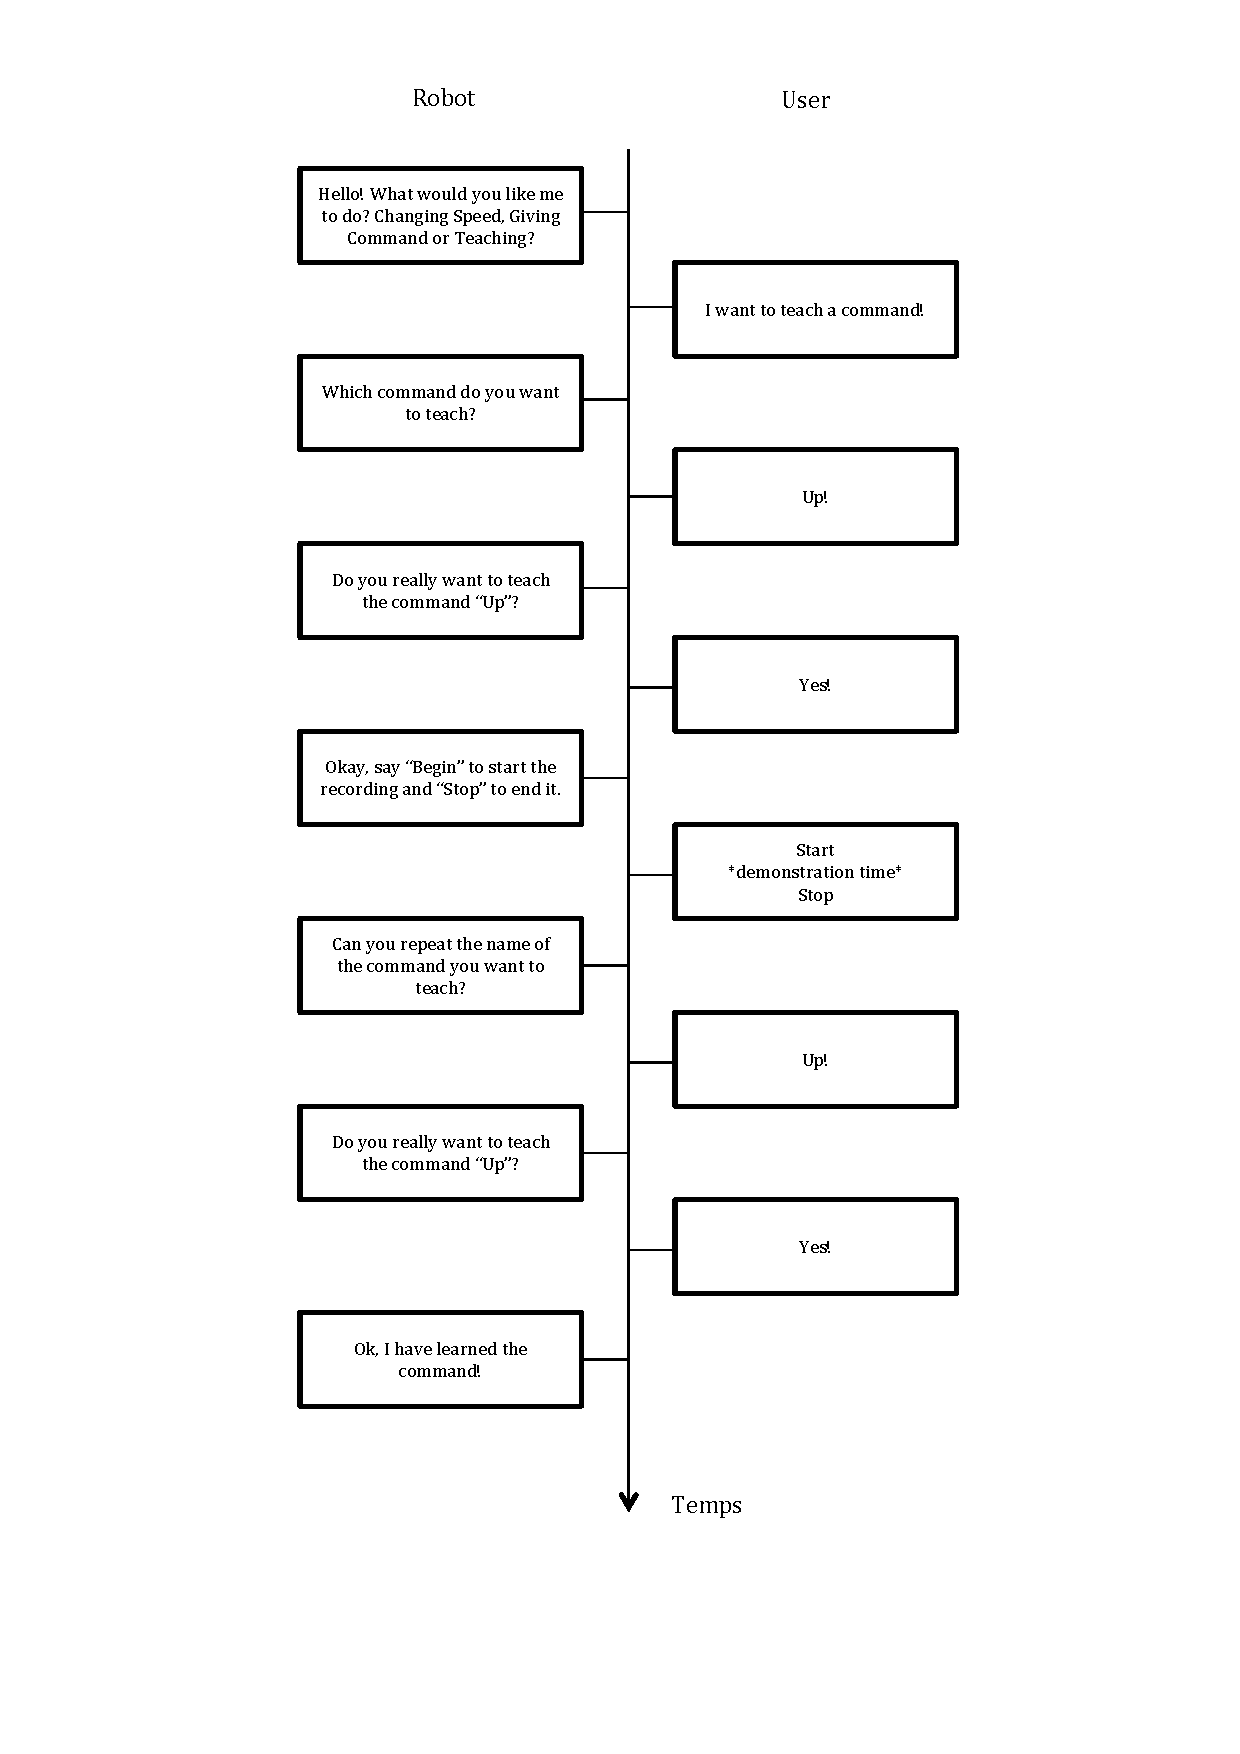
\includegraphics[width=16cm]{img/Schema_Dialogue_TeachingBranch.pdf}\\
\caption{Teaching Command Branch}
\end{center}
\end{figure}

\begin{figure}
\begin{center}
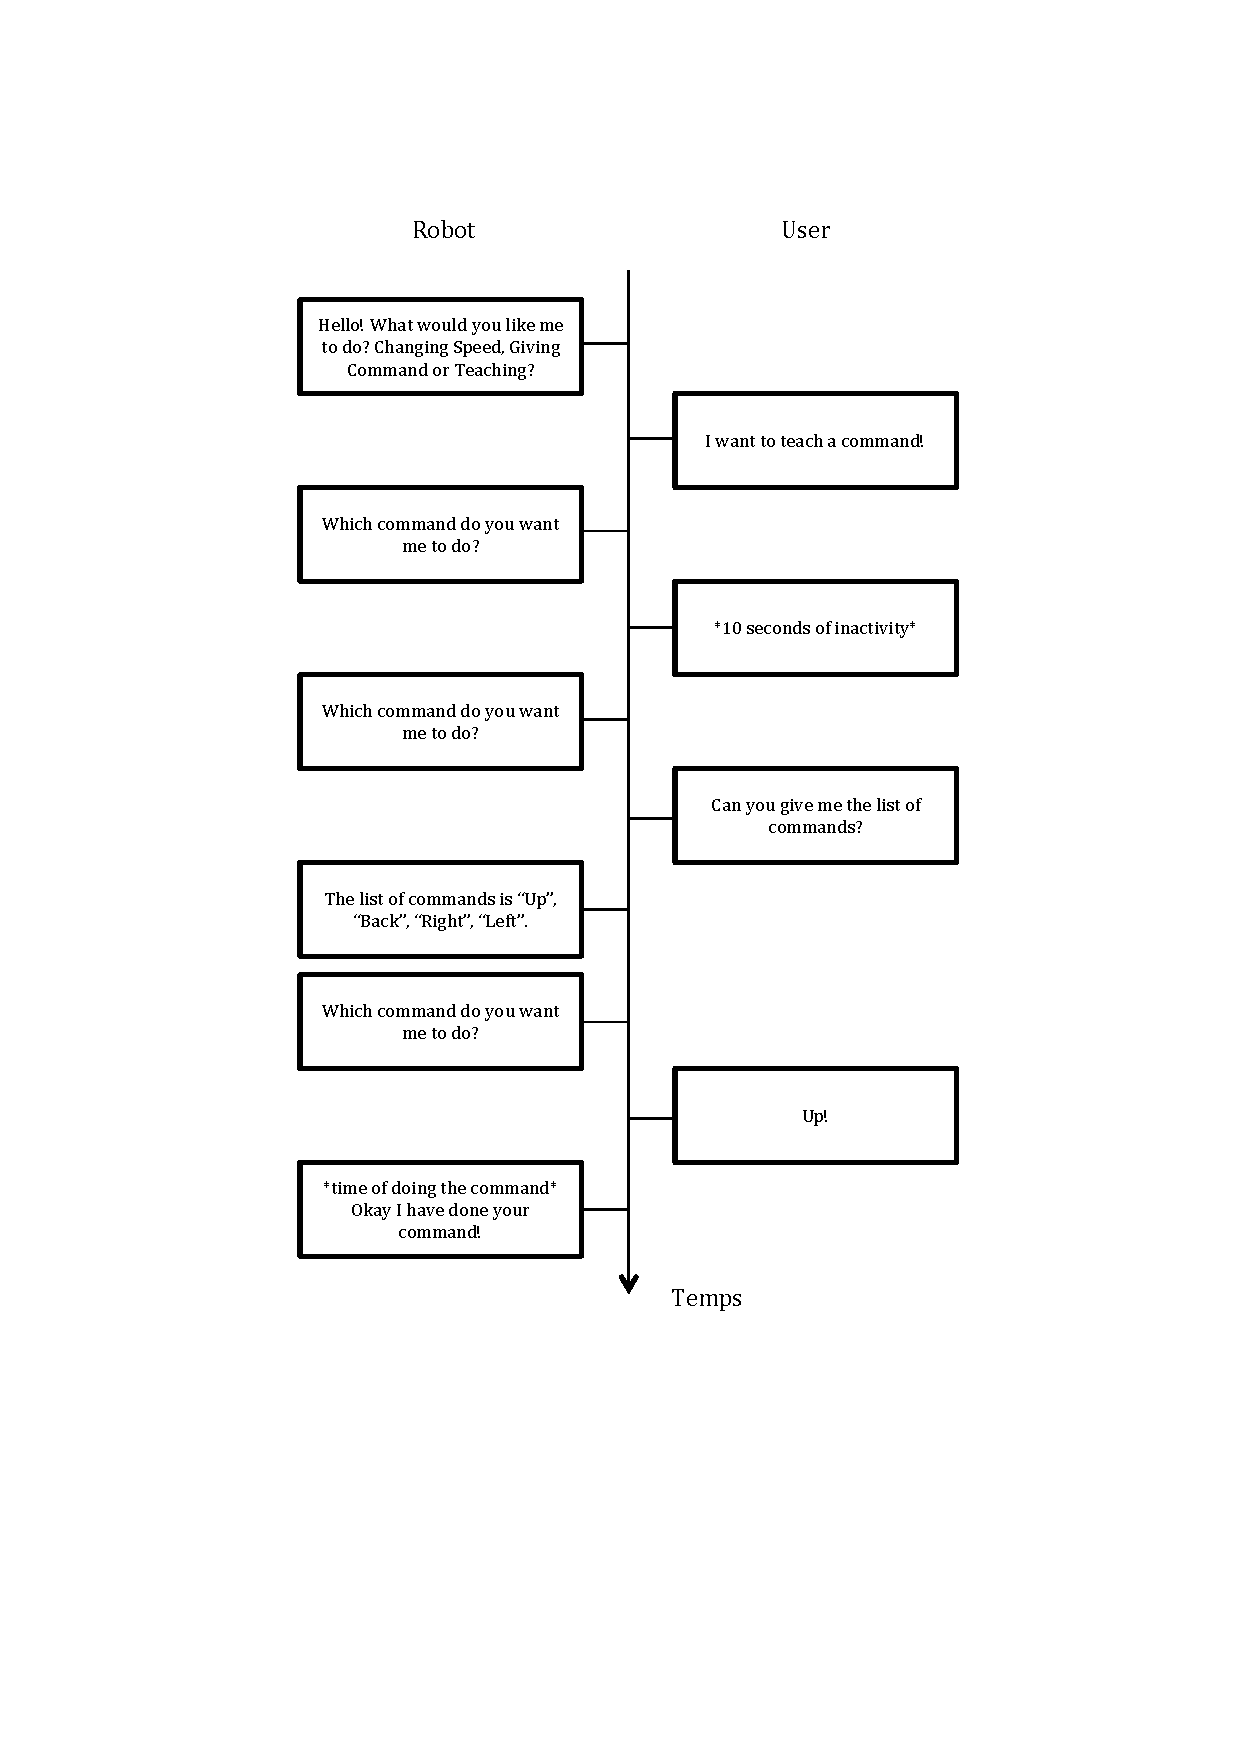
\includegraphics[width=16cm]{img/Schema_Dialogue_CommandingBranch.pdf}\\
\caption{Giving Command Branch}
\end{center}
\end{figure}

\begin{figure}
\begin{center}
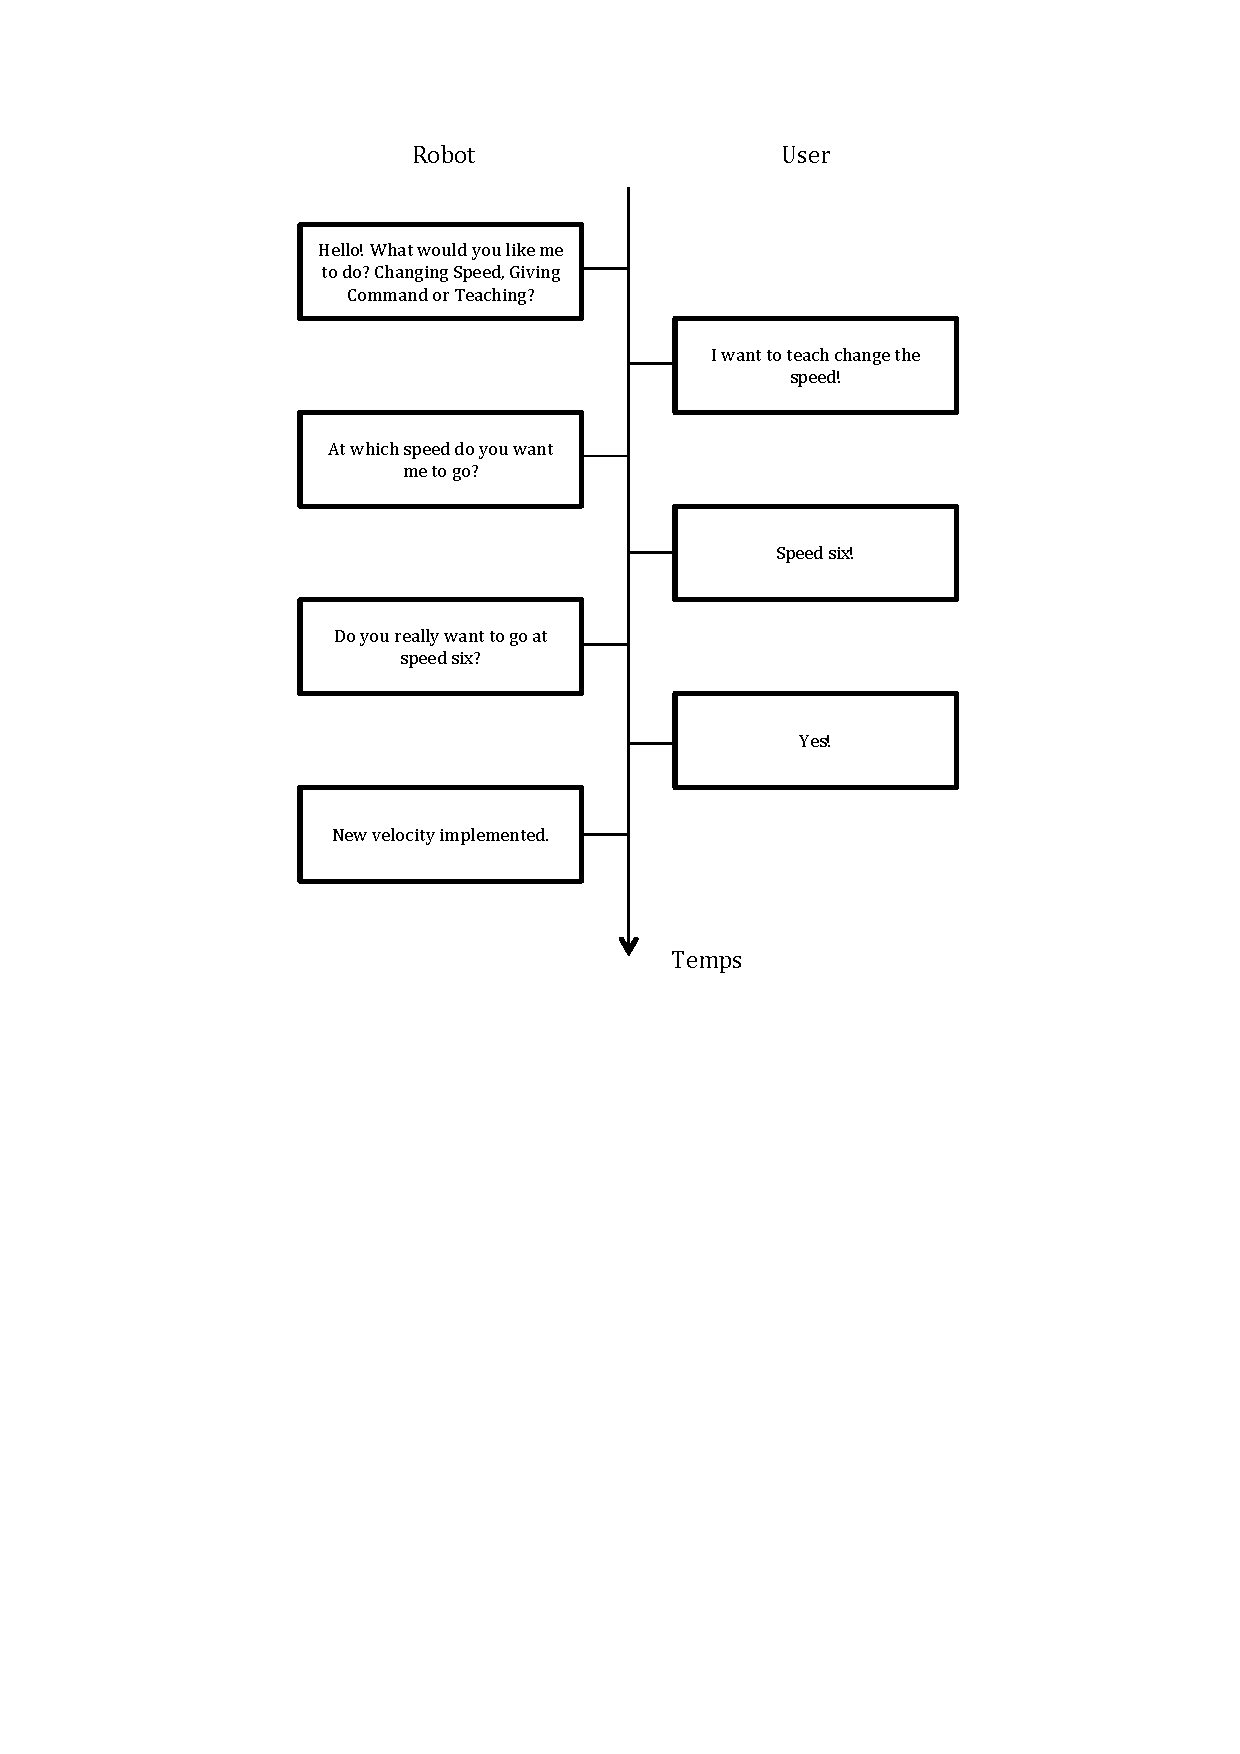
\includegraphics[width=16cm]{img/Schema_Dialogue_SpeedingBranch.pdf}\\
\caption{Changing Speed Branch}
\end{center}
\end{figure}